En aquest capítol s'exposaran les decisions presses a nivell de disseny, tant
d'arquitectura com hardware escollit i programació de la capa de seguretat. Es
continuarà amb l'anàlisi dels components de lògica prograble i d'arquitectura
de codi desenvolupat.

\subsection{ Proposta de disseny }
{
    Per a la implementació del control s'ha decidit utilitzar una arquitectura
    dual basada en lògica programable i en microprocessador. La decisió
    d'implementar el control en lògica programable en comptes d'utilitzar una
    arquitectura basada únicament en microprocessador o FPGA es justifica
    principalment per tres motius.

    En primer lloc, treballar amb una placa d'evaluació que incorpori aquesta
    arquitectura ens permet tenir més flexibilitat quan al disseny, poguent
    decidir si implementar un nou component en software o hardware segons
    evolucioni el projecte. Aquesta major flexibilitat de disseny és força
    interessant en el projecte de l'inversor, ja que permet, per exemple, la
    millora constant de l'algorisme de control per part de futurs membres.

    En segon lloc, la FPGA permet disposar de paral·lelisme real i
    temporització precisa, característiques que es tornen molt atractives en
    augmentar la freqüència de conmutació de l'inversor, sobretot fent servir
    MOSFETs SiC que poden treballar a altes freqüències. Actualment l'inversor
    està dissenyat per conmutar a 16 kHz, però la implementació en FPGA permet
    arribar a freqüències superiors que serien difícils d'assolir implementant
    l'algorisme de control en microcontrolador o microprocessador. De fet, amb
    FPGA es pot arribar inclús a aplicar un control en temps real.

    Finalment, en últim lloc, l'arquitectura de processador permet un
    desenvolupament més ràpid de les parts que no necessiten la velocitat i
    paral·leldismee la FPGA, ja que la descripció de lògica en hardware és més
    vulnerable a errades de programació i les eines de depuració i simulació no
    son tan potents com en software. Per aquesta raó es programa en software la
    interfície d'usuari, la comunicació amb la resta del vehicle i el
    monitoreig de sensors.

    No obstant, s'ha de tenir en compte que l'arquitectura dual també presenta
    inconvenients. La major contrapartida prové de la dificultat de la
    programació de la FPGA i la gestió de la comunicació entre la FPGA i el
    microprocessador. Això es degut principalment a la complexitat i opacitat
    en quan a documentació de les eines de desenvolupament en FPGA com és
    Vivado. Aquestes eines són majoritàriament propietàries i tancades; per
    tant, depenen de la dodumentació lliurada pel fabricant. En conseqüència,
    es prevenen dificultats en la transmissió del coneixement. És per això que
    s'ha posat especial interès als fluxos de treball i l'arquitectura de la
    FPGA, sent aquest un front no totalment resolert en el moment de
    l'escriptura la memòria.

    Seguint aquests motius es decideix utilitzar un SoC que incorpori aquesta
    arquitectura dual. L'avantatge respecte a un SoM és que en estar tots els
    dispositius (FPGA, microprocessadors, memòria i inclús ADCs) en un mateix
    xip la velocitat de comunicació entre aquests és molt reduida, permetent
    una operació a freqüències més altes. Addicionalment, es millora el consum
    energètic en ser dispositius més petits associats al mateix xip.

    No obstant això, l'equip no compta amb els coneixements ni els recursos per
    realitzar una placa d'acondicionament i adaptació d'un SoC. Per aquesta
    raó, es va decantar per utilitzar una placa de desenvolupament comercial.
}

\subsection{ Placa de desenvolupament }
{ 
    A l'inici del projecte, l'equip disposava d'una placa de desenvolupament
    Diligent Cora Z7-10, basada en el \ac{SoC} Zynq-7010 de Xilinx. Amb aquesta
    placa es va arribar a realitzar el testeig dels senyals dels Gate Drivers
    montats en placa \cite{coraz7} \cite{mikel}.

    \begin{figure}[!htb]
        \centering
        \begin{minipage}[c]{8cm}
            \centering
            \captionsetup{justification=centering}
            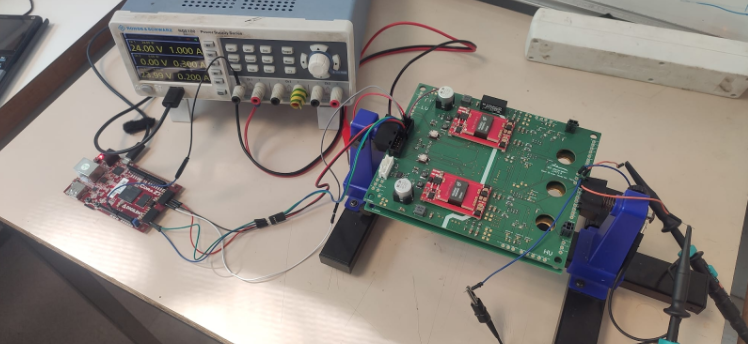
\includegraphics[width=8cm]
                { img/4_implementacio/cora_mikel.png }
            \caption{ La Cora Z-7 en la prova dels Gate Drivers. \emph{BCN eMotorsport.} }                
        \end{minipage} \hfil
        \begin{minipage}[c]{7.5cm}
            \centering
            \captionsetup{justification=centering}
            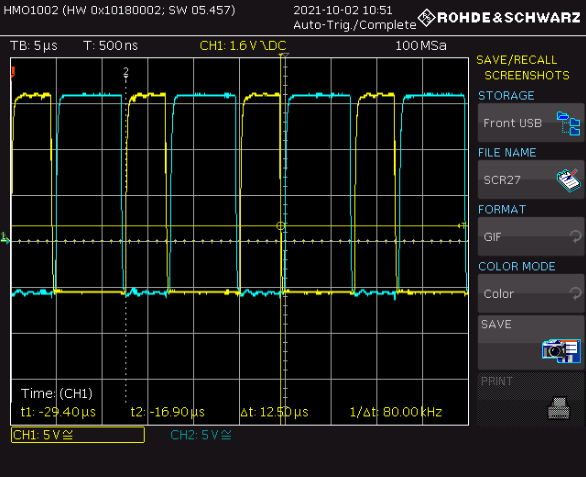
\includegraphics[width=5.5cm]
                { img/4_implementacio/gate_drivers.png }
            \caption{ Captura de l'oscil·loscopi. \emph{BCN eMotorsport.} }                
        \end{minipage} \hfil
    \end{figure} 

    De cara a una implementació futura de l'inversor, es va decidir substituir
    la Cora Z7-10 per una placa que facilités el desenvolupament de l'inversor
    i que millorés la implementació final de l'inversor de cara a l'any vinent.
    Es volia trobar una placa amb més recursos lògics i un major nombre
    d'entrades de propòsit general (GPIO) per poder implementar el control pels
    quatre motors en la mateixa placa. També es va procurar que la
    documentació fos bona i extensa.

    El primer que es va pensar es si continuar amb el mateix fabricant del SoC,
    Xilinx. Després d'un anàlisi de la competència, es va veure que Xilinx
    continuava sent la millor opció: 
    
    \begin{itemize}
        \item
            Es tracta del major fabricant de FPGAs en l'actualitat, amb una
            quota de mercat per facturació superior al 50\%, desbancant als
            seus competidors com són Altera d'Intel o Lattice. En conseqüència,
            la comunitat al voltant els seus productes és més extensa i és més
            senzill trobar recursos de consulta.
        \item 
            L'equip ja disposava d'un \emph{know-how} de l'ús de les eines de
            desenvolupament de Xilinx, en específic de la suite
            Vitis/Vivado\textsuperscript{\textregistered}. Es tracten d'eines
            bastant complexes i intimidants en un principi, però resulten ser
            potents en quan a funcionalitat.
    \end{itemize}

    Finalment es va decidir comprar la Z-Turn del fabricant Make Your Idea
    Real, que era una de les poques plaques disponibles degut a l'actual falta
    de stock de components electrònics, en especial semiconductors. Compleix
    les especifiacions demanades a un preu competitiu. Com que la família de
    SoC es la mateixa, gran part del \emph{know-how} del equip és aplicable a
    la nova placa \cite{zturn}.

    \begin{figure}[!htb]
        \centering
        \begin{minipage}[c]{7cm}
            \centering
            \captionsetup{justification=centering}
            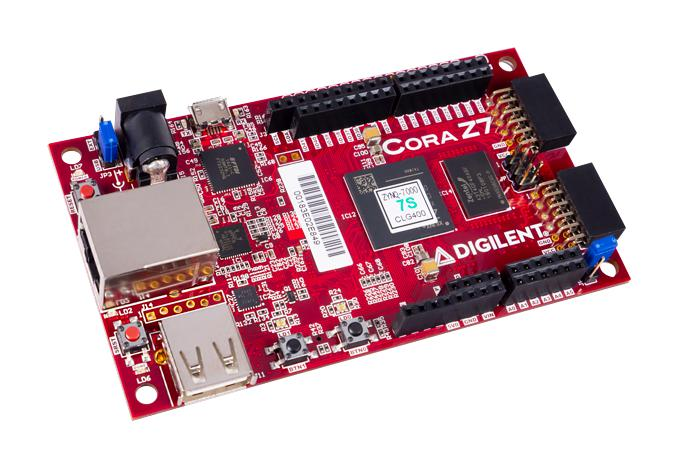
\includegraphics[width=7cm]
                { img/4_implementacio/cora-z7.jpg }
            \caption{ Digilent Cora Z7-10 }                
        \end{minipage} \hfil
        \begin{minipage}[c]{7cm}
            \centering
            \captionsetup{justification=centering}
            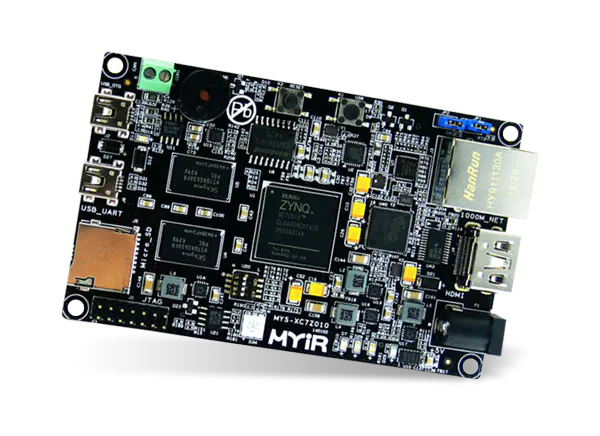
\includegraphics[width=6.5cm]
                { img/4_implementacio/zturn.png }
            \caption{ MIYR Z-Turn }                
        \end{minipage} \hfil
    \end{figure} 

    \begin{table}[!htb]
        \caption{ Comparativa entre la Digilent Cora Z7-10 i la MYIR Z-Turn }
        \centering
        \tablefirsthead{}
        \tablehead{}
        \tabletail{}
        \tablelasttail{}
        \renewcommand{\arraystretch}{1.3}
    
        \begin{supertabular} {|l|l|m{4.5cm}|m{4.5cm}|}
            \hline
                \multicolumn{2}{|l|}{ \textbf{ SoM } } & 
                \textbf{ Digilent Cora Z7-10 } & 
                \textbf{ MYIR Z-Turn } \\
            \hhline{|=|=|=|=|} \multirow{10}{*}{ SoC } & 
                { Família } & \multicolumn{2}{|c|}{ Xilinx Zynq-7000 } \\
            \cline{2-4} &
                { Model } &
                    { Z-7010 XC7Z010 } & 
                    { Z-7020 XC7Z020 } \\
            \cline{2-4} &
                { Microprocessador } & 
                    \multicolumn{2}{|c|}{ ARM Cortex-A9 de 2 nuclis } \\
            \cline{2-4} & 
                { Slices } &
                    { 4.400 } & 
                    { 13.300 } \\
            \cline{2-4} & 
                { Blocs \acs{DSP} dedicats } &
                    { 80 } & 
                    { 220 } \\
            \cline{2-4} & 
                { Look-Up tables (LUTs) } &
                    { 17.600 } & 
                    { 53.200 } \\
            \cline{2-4} & 
                { Flip-flops } &
                    { 35.200 } & 
                    { 106.400 } \\
            \cline{2-4} & 
                { Block RAM } &
                    { 2.1 Mb (60 blocks) } & 
                    { 4.9 Mb (140 blcks) } \\
            \cline{2-4} & 
                { Freq. de rellotge màx. } & \multicolumn{2}{|c|}{ 667 MHz } \\
            \cline{2-4} & 
                { ADC } & \multicolumn{2}{|c|}{ 2x 12 bits ADC @ 1 MSPS } \\
            \hhline{|=|=|=|=|}
                \multicolumn{2}{|l|}{ Memory } &
                { 
                    \medskip     
                    512 MB DDR3 SDRAM \newline (16-bit bus) \newline
                    SD card slot
                } &
                { 
                    \medskip 
                    1 GB DDR3 SDRAM \newline (32-bit bus) \newline
                    SD card slot
                } \\            
            \hline            
                \multicolumn{2}{|l|}{ Connectors } &
                { 
                    \medskip 
                    61x user GPIO \newline
                    1x USB-UART \newline
                    1x JTAG for debbuging \newline
                    1x Ethernet \newline
                    2x Pmod connectors \newline
                    \newline
                } &
                {  
                    \medskip
                    106x user GPIO \newline
                    1x USB-UART \newline
                    1x JTAG for debbuging \newline
                    1x Ethernet \newline
                    1x CAN \newline
                    1x HDMI
                } \\
            \hline
                \multicolumn{2}{|l|}{ Dispositius configurables } &
                { 
                    \medskip 
                    2x Botó polsador \newline
                    2x RGB LEDs \newline
                } &
                {  
                    \medskip 
                    1x Botó pulsador \newline
                    1x RGB LED \newline
                    1x Bruncidor
                } \\
            \hline
                \multicolumn{2}{|l|}{ Entrades d'alimentació } &
                { 
                    \medskip 
                    USB \newline
                    Font externa de 5V
                } &
                { 
                    \medskip 
                    USB \newline
                    Font externa de 5V
                } \\
            \hline
                \multicolumn{2}{|l|}{ Dimensions } &
                    { $57.9\ mm \times 101.6\ mm $  } & 
                    { $63.0\ mm \times 102.0\ mm $ } \\
            \hline
                \multicolumn{2}{|l|}{ Preu } &
                    { 127,45€ } &
                    { 187,72€ } \\
            \hline
        \end{supertabular}
    \end{table}

    Un cop escollida la placa de desenvolupament, s'ha de decidir en funció
    dels recursos de hardware disponibles quina part del control es realitza en
    lògica programable i quina en processador:

    \begin{itemize}
        \item \textbf{Lògica programable:} 
            Es programarà en l'algorisme de control des de les consignes de
            velocitat i parell fins a la generació del PWM, inclosa la
            incorporació del deadtime per als Gate Drivers. Això inclou la
            lectura de les mesures de corrent que arriben a la placa en forma
            de PWM i les lectures d'angle i velocitat del resolver.

        \item \textbf{Processador:}
            Es programarà la màquina d'estats per controlar l'arrencada i la
            parada del motor, la interfície de testeig en pantalla i la
            comunicació amb la resta del vehicle per mitjà de bus CAN. Això
            inclou una comunicació amb la PU per rebre les consignes de
            velocitat i parell, i la comunicació amb la placa de precàrrega
            dels condensadors de l'inversor.

    \end{itemize}
}

\subsection{ Implementació de l'algorisme de control }
{
    Per implementar la lògica programable es decideix utilitzar \emph{Vitis
    Model Composer}, una extensió de Matlab/Simulink\textsuperscript{\textregistered}
    que proporciona un \emph{blokset} amb el qual descriure i implementar la lògica
    programable. Anteriorment a 2019, l'eina es comercialitzava baix el nom de
    \emph{System Generator}, per la qual cosa encara apareix aquest nom en
    bastanta documentació. El \emph{blockset} incorpora blocs estàndard de
    \ac{DSP}, com poden ser sumadors-restadors, multiplexors, productes,
    multiplicacions per constants i look-up tables, a més de diversos blocs per
    truncar i transformar tipus de dades. 

    La decisió d'utilitzar aquest entorn \emph{low-code} en comptes d'escriure
    codi en llenguatge de descripció de hardware, per exemple \acs{VHDL}, es
    justifica amb una major velocitat de desenvolupament i testeig degut a la
    integració directa amb Matlab/Simulink\textsuperscript{\textregistered}. Es
    poden fer servir els models desenvolupats amb anterioritat per l'equip per
    validar el funcionament de la programació. La progamació \emph{low-code}
    pot resultar més atractiva en un principi; no obstant, no eximeix de tenir
    coneixements de disseny de lògica digital.
    
    La freqüència de rellotge escollida pel sistema és de 10 ns, molt superior
    al de la freqüència de commutació de l'inversor, de 16 kHz. Això permet
    temptejar amb un control en temps real, és a dir, sense modelar l'efecte
    del retard del processament de l'algorisme i millorar les prestacions del
    control, cosa que seria difícil d'aconseguir amb un microcontrolador.
    
    En quan a tipus numèric a emprar, s'ha decidit fer servir coma fixa, ja que
    és menys exigent en termes de recursos que la coma flotant; no obstant
    això, la dificultat de la implentació es veu augmentada en haver de
    realitzar un seguiment de la mida del tipus numèric en cada bloc
    implementat. Les mides de la coma fixa utilitzades es recullen a l'annex
    \ref{fixed_point}. Com norma general, s'ha introduit pipelining per tal de
    reduir el consum dinàmic del control \cite{power_fpga}.

    En les següents subseccions s'analitzaran els diversos blocs implementats.

    \begin{figure}[!htb]
        \centering
        \captionsetup{justification=centering, margin=1.5cm}
        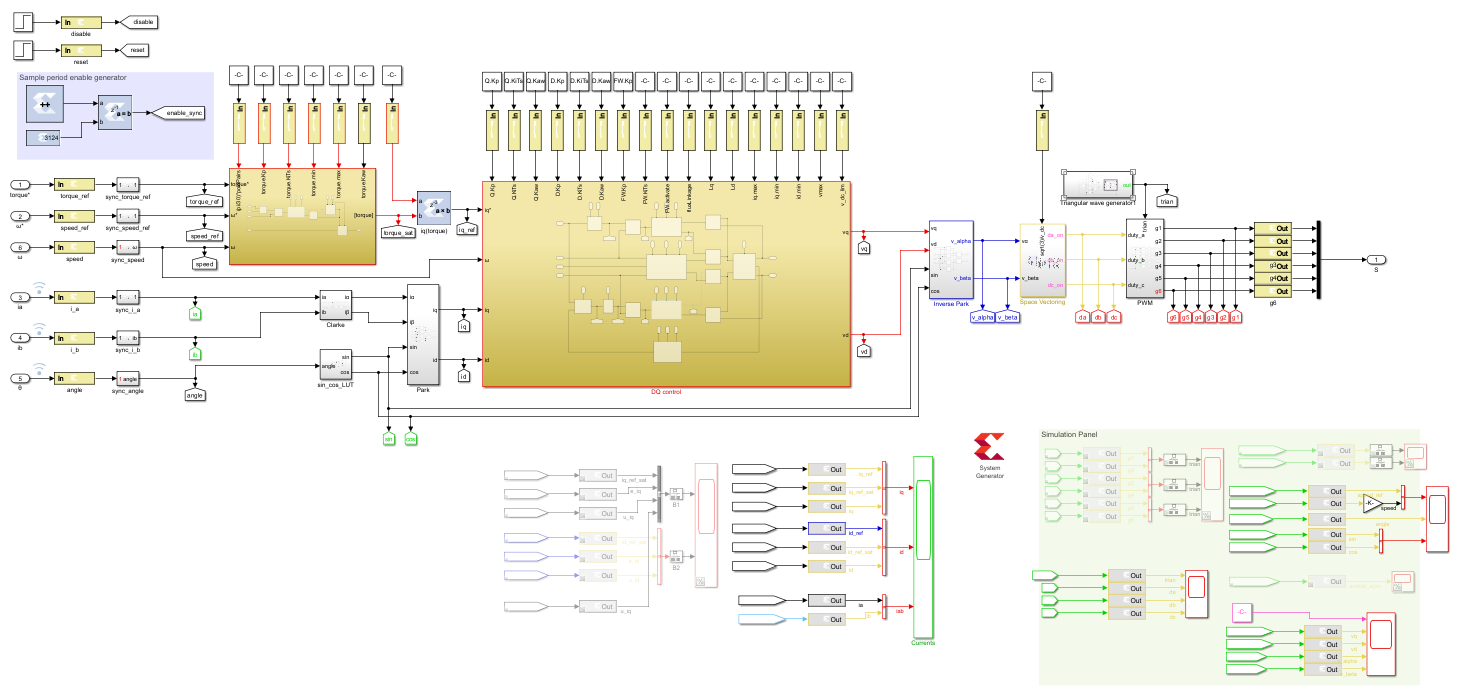
\includegraphics[width=16cm]
            { img/4_implementacio/control.png }
        \caption{ Implementació del control amb Vitis\texttrademark Model Composer }
    \end{figure}

    \subsubsection{ Controladors PI }
    { 
        L'algorisme fa servir un total de quatre controladors
        proporcionals-integrals (PI) ajustats manualment. S'ha decicit
        utilitzar controladors PI en comptes de PID perquè la part derivativa
        del control pot arribar a comportar-se erràticament en contextes amb
        molt de soroll. Els PI del control de corrent compten amb
        \emph{anti-windup}, ja que en cas contrari els PI calcularien els
        següents valors sense saber que la seva resposta està saturada. La
        tècnica de wind-up implementada consisteix a multiplicar per una
        constant l'error degut a la saturació i sumar-ho a l'acummulador del
        control integral \cite{pi_fpga}.

        \begin{figure}[!htb]
            \centering
            \captionsetup{justification=centering, margin=1.5cm}
            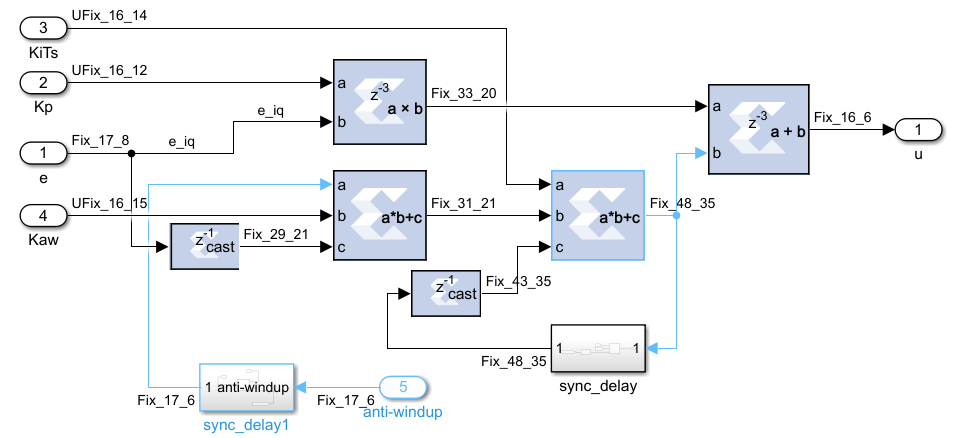
\includegraphics[width=11cm]
                { img/4_implementacio/PI_controller_id.png }
            \caption{ Detall de la implementació d'un PI amb \emph{anti-windup} }
        \end{figure}
    }

    \subsubsection{ Control de velocitat }
    { 
        La implementació del control de velocitat es basa en una doble
        saturació de la consigna de parell. L'estimació del límit superior del
        parell es realitza amb un controlador PI l'entrada del qual és l'error
        en la velocitat angular actual.

        \begin{figure}[!htb]
            \centering
            \captionsetup{justification=centering, margin=1.5cm}
            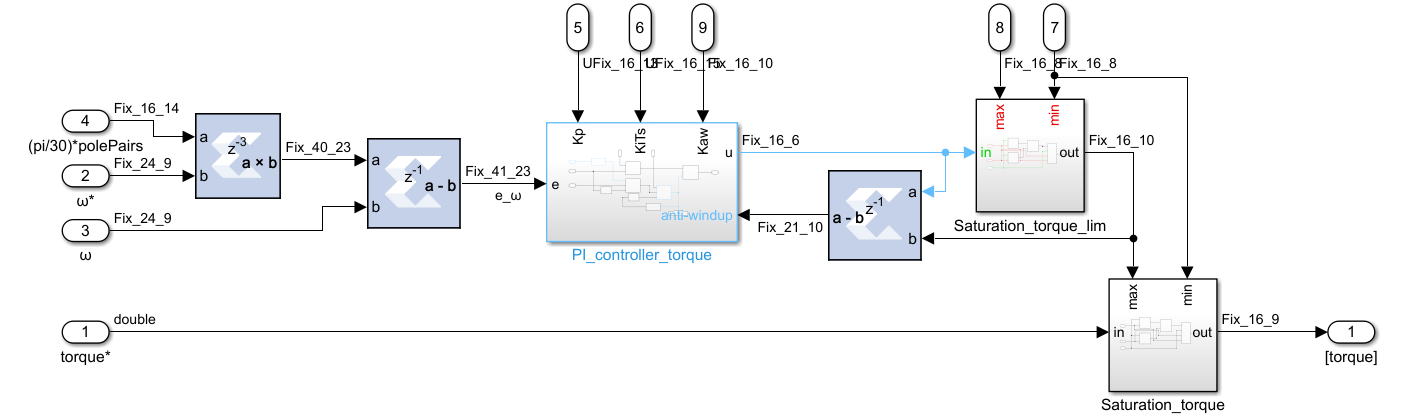
\includegraphics[width=14cm]
                { img/4_implementacio/speed_control.png }
            \caption{ Implementació del control de velocitat }
        \end{figure}
    }

    \subsubsection{ Sinus i cosinus }
    { 
        Per obtenir el sinus i el cosinus d'un angle donat, necessari per
        implementar la transformada i la antitransformada de Park, s'ha
        inclòs una look-up table amb els seus valors i una certa lògica
        addicional que permet la multiplexació de la lookup table per obtenir
        simultàniament ambdues funcions trigonomètriques.

        \begin{figure}[!htb]
            \centering
            \captionsetup{justification=centering, margin=1.5cm}
            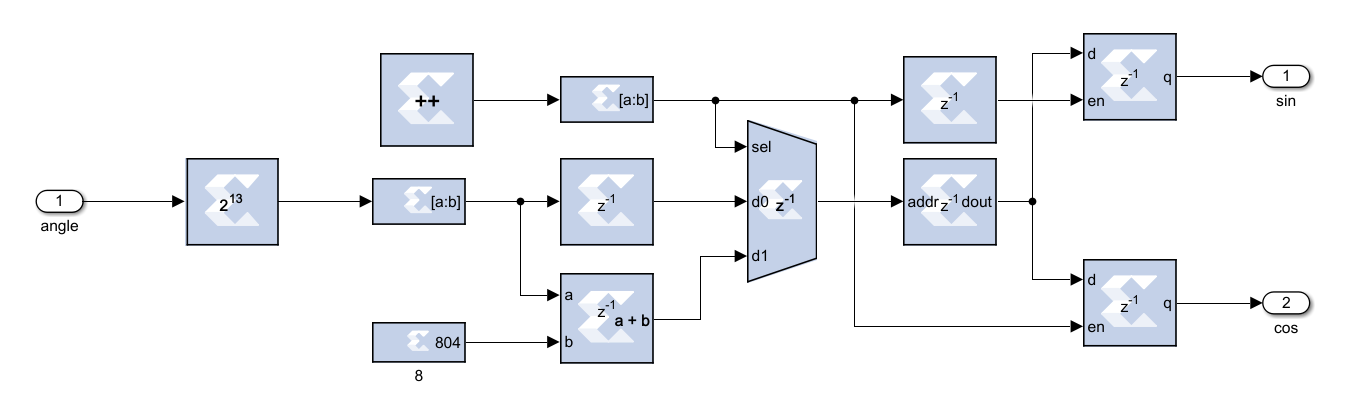
\includegraphics[width=12cm]
                { img/4_implementacio/sineLUT.png }
            \caption{ Implementació de les funcions sinus i cosinus }
        \end{figure}
    }

    \subsubsection{ Transformades de Clarke i de Park }
    { 
        La implementació de la transformada de Clarke és relativament senzilla,
        ja que es tracta d'una transformació lineal. Per tant, es pot expressar
        en termes de sumes i multiplicacions. És convenient recalcar que la
        multiplicació per una potència de 2 no comporta penalització de
        recursos de hardware utilitzats, ja que en aritmètica de coma flotant
        aquesta operació es pot realitzant simplement reinterpretant la
        posición de la coma fixa.

        La transformada de Park, per la seva banda, s'ha implementat amb quatre
        blocs multiplicadors i 2 blocs sumadors-restadors.

        \begin{figure}[!htb]
            \centering
            \begin{minipage}[c]{7cm}
                \centering
                \captionsetup{justification=centering}
                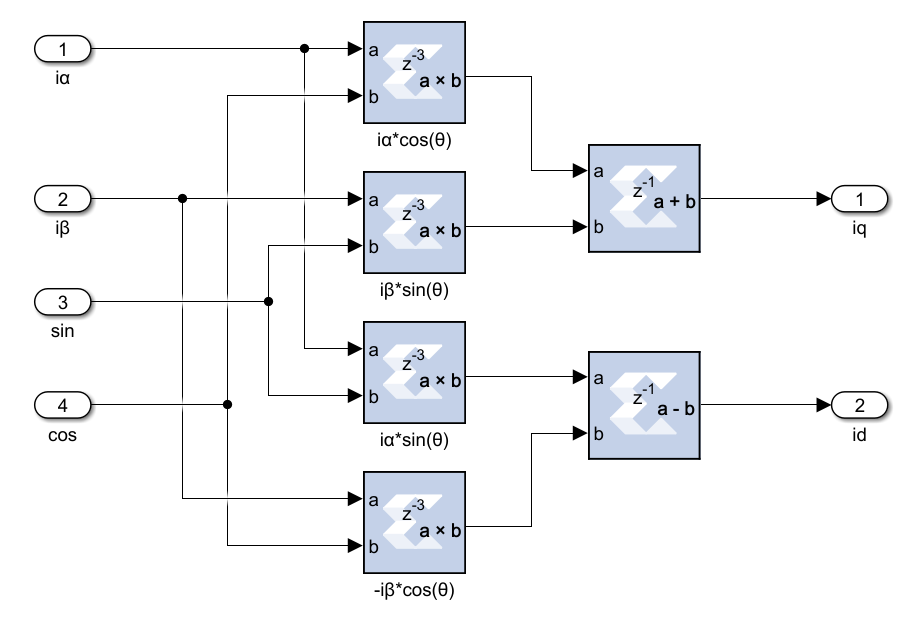
\includegraphics[width=7cm]
                    { img/4_implementacio/park.png }
                \caption{ Implementació de la transformada de Park }        
            \end{minipage} \hfil
            \begin{minipage}[c]{7cm}
                \centering
                \captionsetup{justification=centering}
                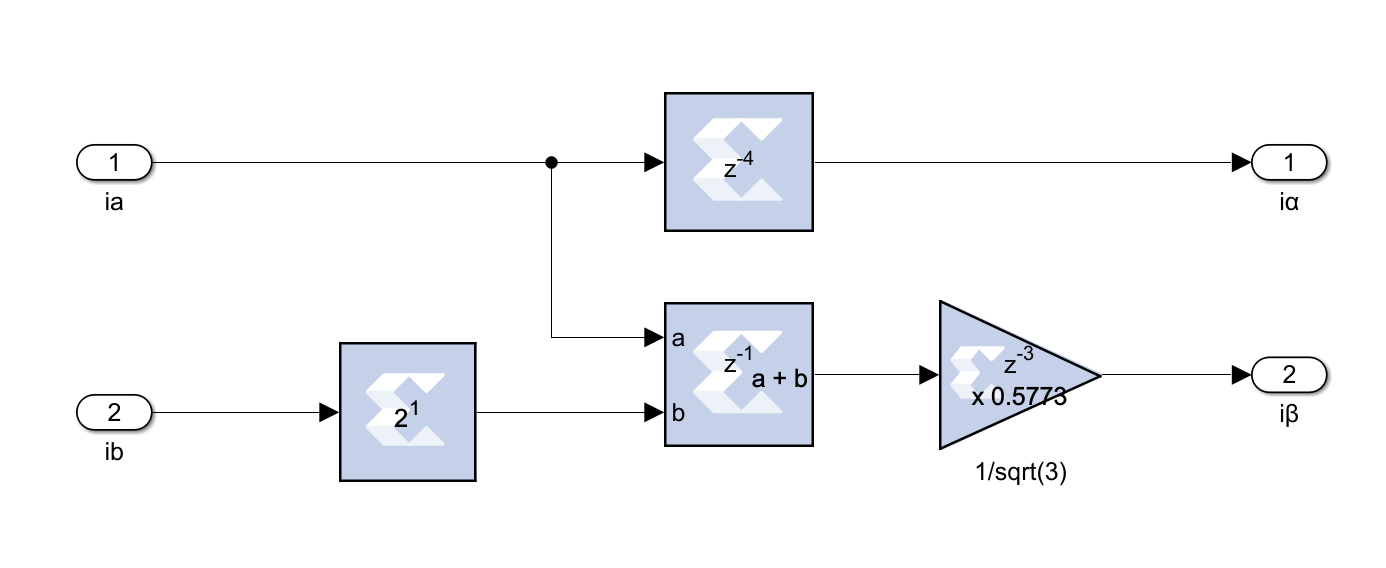
\includegraphics[width=7cm]
                    { img/4_implementacio/clarke.png }
                \caption{ Implementació de la transformada de Clarke }           
            \end{minipage} \hfil
        \end{figure} 
    }

    \subsubsection{ Control de corrent }
    { 
        Per al control de corrent s'han implementat dos controladors
        proporcionals-integrals (PI) ajustats manualment. En el mateix bloc
        també s'han implementat les funcions de desacoblament i de el limitador
        de voltatge, que limita la magnitud del voltage; així com les
        corresponents al Field Weakening i el MTPA.

        \begin{figure}[!htb]
            \centering
            \captionsetup{justification=centering, margin=1.5cm}
            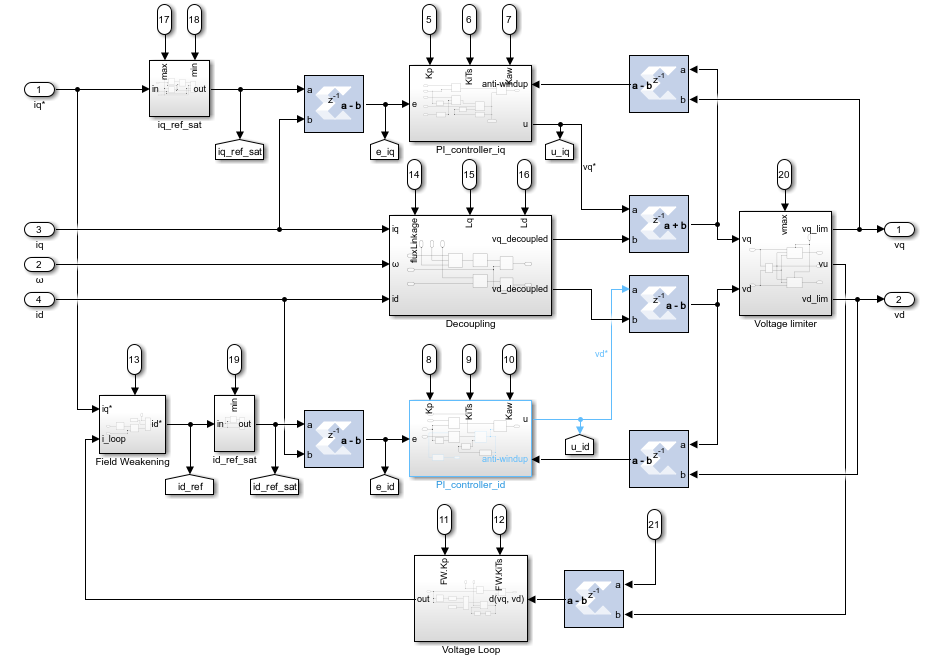
\includegraphics[width=12cm]
                { img/4_implementacio/current_control.png }
            \caption{ Vista general del bloc de control de corrent }
        \end{figure}
    }

    \subsubsection{ Field Weakening }
    { 
        El debilitament de camp s'implementa com un llaç de control tancat amb
        un controlador PI semblant als del control de corrent. No obstant,
        compta amb una condició inicial que ha de complir per activar el seu
        funcionament. Per tal d'activar el Field Weakening, per una banda, la
        velocitat ha de ser superior a la velocitat base, que és de 9000 rpm, i
        per l'altra, el voltatge de referència calculat ha de ser superior al
        de bus DC. Aquest bloc es pot desactivar si el senyal FW.activate es
        posa a 0.
    
        \begin{figure}[!htb]
            \centering
            \captionsetup{justification=centering, margin=1.5cm}
            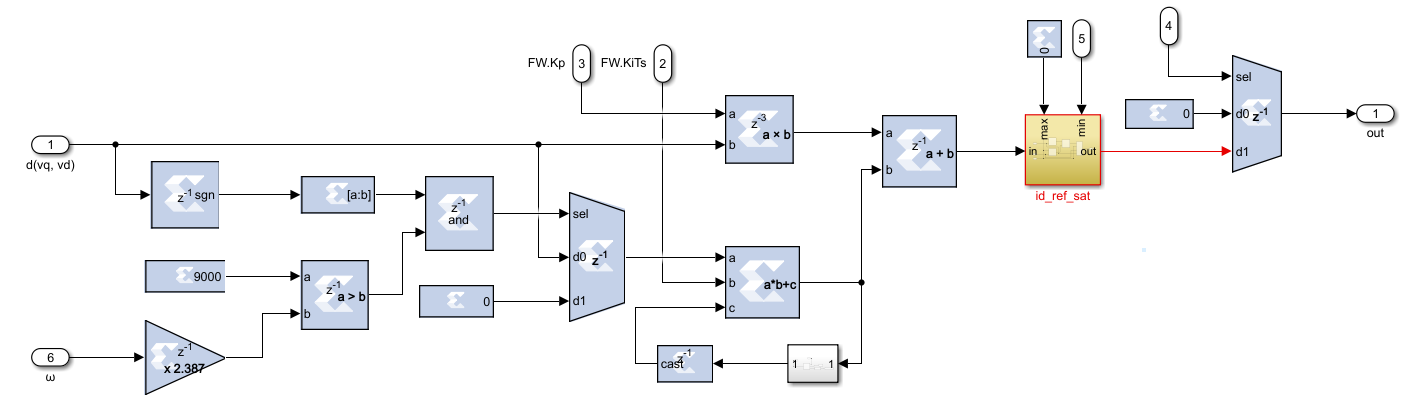
\includegraphics[width=14cm]
                { img/4_implementacio/fw.png }
            \caption{ Implementació del Field Weakening }
        \end{figure}
    }

    \subsubsection{ MTPA i generació de la referència $i_d*$ }
    { 
        El bloc de generació de la referència de corrent $i_d*$ rep a les
        entrades del llaç de voltatge del Field Weakening i realitza el càlcul
        del MTPA. L'equació de MTPA s'ha implementat per mitjà d'una look-up
        table i, a l'igual que el bloc de FW, compta amb un multiplexor per
        activar o desactivar aquesta estratègia de control.

        \begin{figure}[!htb]
            \centering
            \captionsetup{justification=centering, margin=1.5cm}
            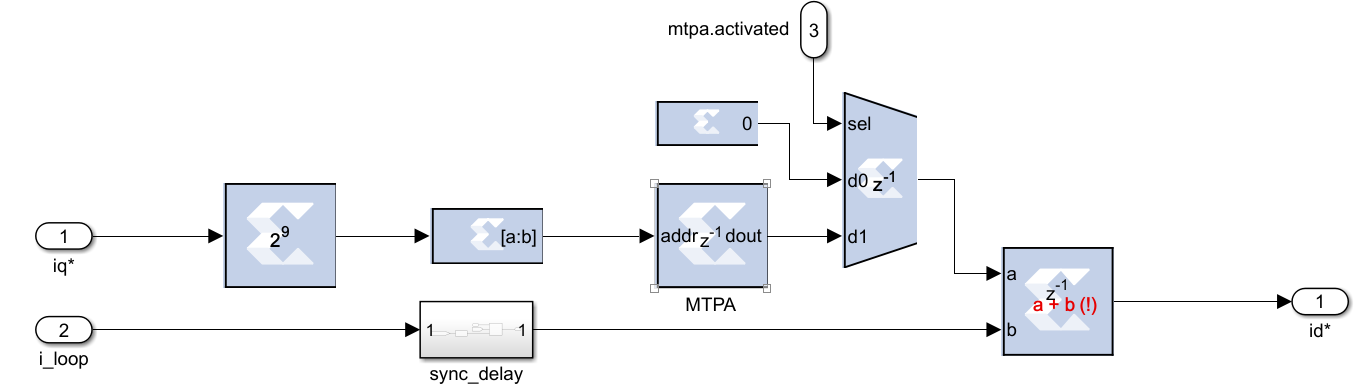
\includegraphics[width=12cm]
                { img/4_implementacio/mtpa.png }
            \caption{ Implementació de la generació del corrent de referència $i_d*$ }
        \end{figure}
    }

    \subsubsection{ Space Vector Modulation }
    { 
        En la figura \ref{ svpwm_fpga } es pot veure que s'han agrupat el
        diferents blocs per funcionalitat. Així, a la part superior, tenim la
        identificació del sector com tres condicions i un bloc concatenador;
        baix a l'esquerra estàn els multiplicadors que realitzen la
        normalització del vector de referència; a la seva dreta, es troben els
        blocs amb els quals obtenim les variables X, -X, Y, -Y, Z i -Z, i
        finalment els blocs generadors dels temps $t_1'$, $t_2'$ i $t_0$,
        associent-los a la fase corresponent de l'inversor per mitjà de tres
        multiplexors. 

        \begin{figure}[!htb]
            \centering
            \captionsetup{justification=centering,margin=1.5cm}
            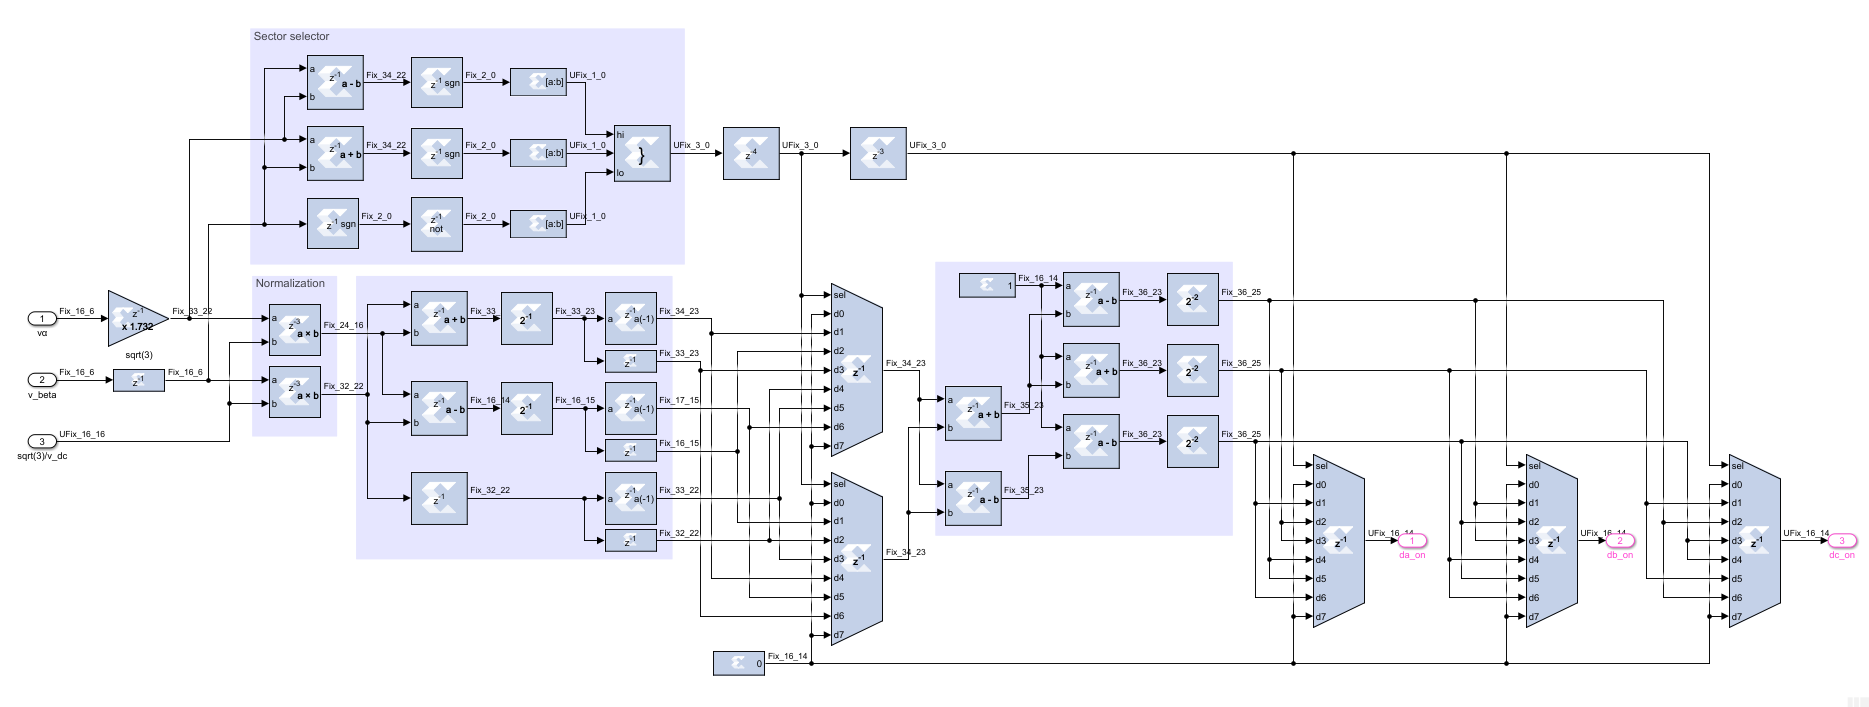
\includegraphics[width=16cm]
                { ../img/4_implementacio/sv.png }
            \caption{ Implementació de l'SVPWM. }
            \label{ svpwm_fpga }
        \end{figure}
    }

    \subsubsection{ Generació de PWM }
    {
        Per generar els senyals de commutació del transistor es comparen els
        tres cicles de treballs aconseguits mitjançant la modulació SV amb una
        portadora triangular. Cada comparació dóna lloc a dos senyals PWM
        contraposats, una l'inversa de l'altre, que corresponen als temps
        d'encesa i d'apagada dels dos transistors d'una fase de l'inversor. És
        important generar un petit temps entre els flancs de pujada i de
        baixada de les tensions de porta del transistors, ja que els pendents
        no són ideals; és el que es coneix com \emph{deadtime}. En el nostre
        cas, implementem un \emph{deadtime} d'$1 \mu s$.

        \begin{figure}[!htb]
            \centering
            \begin{minipage}[c]{7cm}
                \centering
                \captionsetup{justification=centering}
                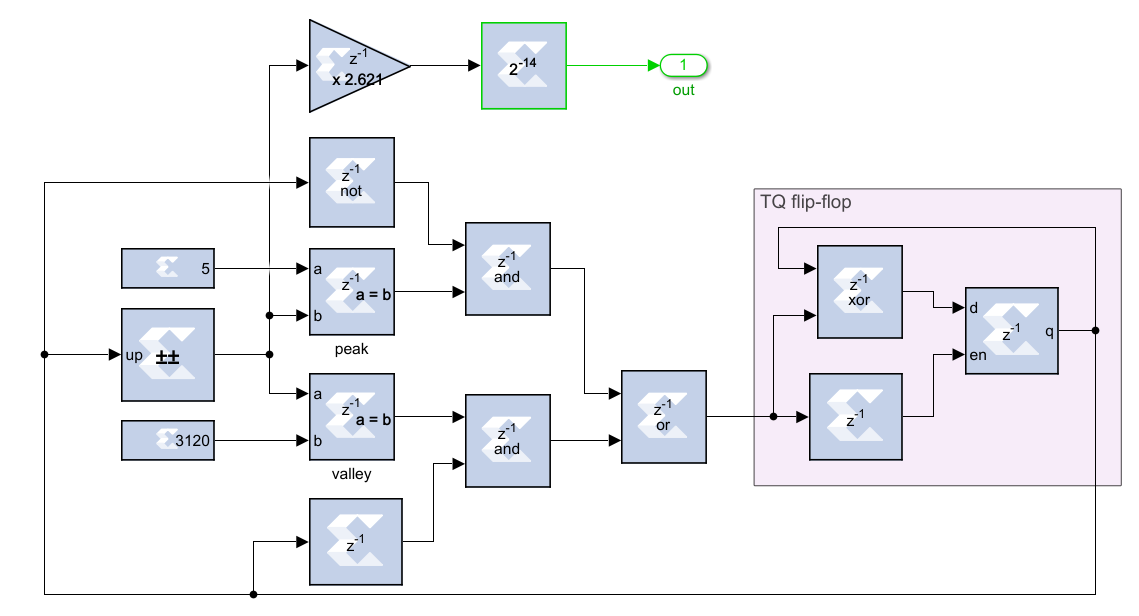
\includegraphics[width=7cm]
                    { img/4_implementacio/triangular.png }
                \caption{ Bloc de generaciió de la portadora triangular }                
            \end{minipage} \hfil
            \begin{minipage}[c]{7cm}
                \centering
                \captionsetup{justification=centering}
                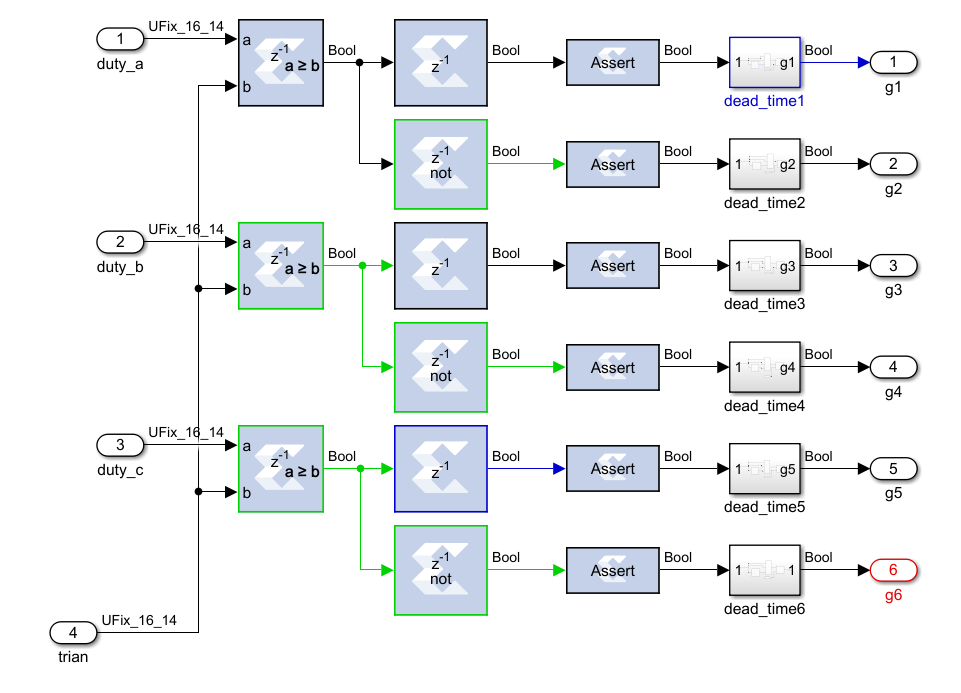
\includegraphics[width=7cm]
                    { img/4_implementacio/pwm.png }
                \caption{ Bloc de generaciió de PWM }                
            \end{minipage} \hfil
        \end{figure} 
    }
}

\subsection{ Implementació de la lògica programable }
{ 
    Un cop validat l'algorisme de control en
    \emph{Matlab/Simulink\textsuperscript{\textregistered}}, s'exporta el model
    a IP de \emph{Vivado}, l'eina de Xilinx per a la programació de les seves
    FPGAs. Les IP (\emph{Intelectual Property}) de \emph{Vivado} són
    subsistemes desenvolupats en aquesta eina que poden ser emprats en altres
    projectes. Xilinx disposa d'una extensa llibreria d'IPs que poden ser
    utilitzades per reduir l'esforç de disseny i el \emph{time to market}.

    Directament des del bloc \emph{System Generator} de \emph{Vitis Model
    Composer} es pot afegir la configuració per generar IPs. En tenir-ho, s'ha
    d'integrar la IP en un projecte de \emph{Vivado}. Per provar les
    funcionalitats de l'algorisme de control sobre la placa, s'ha realitzat el
    següent disseny de blocs de Vivado:

    \begin{figure}[!htb]
        \centering
        \captionsetup{justification=centering,margin=1.5cm}
        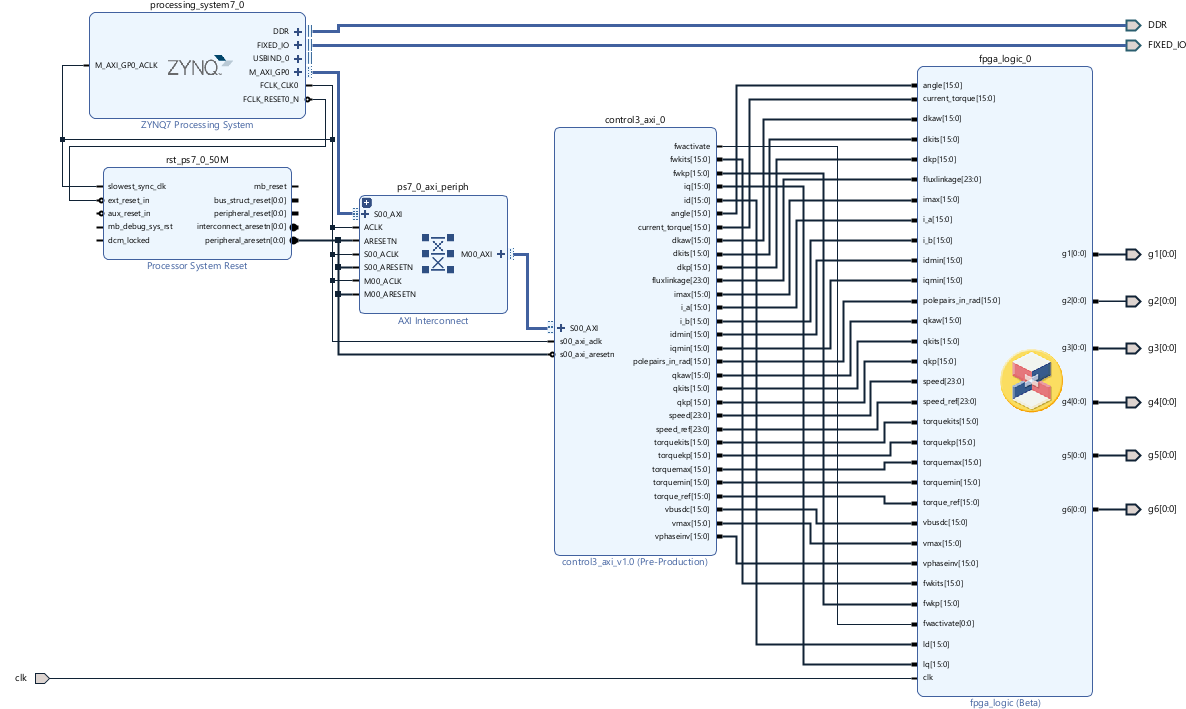
\includegraphics[width=15.5cm]
            { img/4_implementacio/vivado.png }
        \caption{ Disseny de blocs en el projecte de Vivado }
    \end{figure}

    En el cantó superior esquerra es troba el bloc que configura el processador
    del SoC Zynq. Just a la dreta del bloc de reset es troba el bloc que permet
    l'ús del bus \ac{AXI} de comunicació entre la lògica programable i el
    processador. Per configurar els registres del bus \ac{AXI} es fa servir l'IP
    customitzada \emph{control3\_axi} que actua com un perifèric del bus \ac{AXI}.
    Finalment, a la dreta tenim el bloc generat mitjançant l'eina \emph{Vitis
    Model Composer} i que conté l'algorisme desenvolupat.

    Seguint el flux de treball de Vivado, s'ha de realitzar la síntesi i la
    implementació del disseny. Els resultats de la implementació s'adjunten a
    l'annex \ref{vivado}.
}

\subsection{ Implementació del sistema d'arrencada i parada }
{ 
    El sistema d'arrencada i parada s'ha implementat com una aplicació escrita
    en llenguatge C++ que corre a sobre d'una distribució específica de Linux.

    \subsubsection{ Linux }
    { 
        La distribució implementada per al projecte es coneix com PetaLinux,
        està desenvolupada per Xilinx i és específica dels SoCs de la família
        Zynq-7000. 
        
        Linux permet abstreure el desenvolupament d'aplicacions del hardware
        que el suporta. Això es converteix en un avantatge si es vol aconseguir
        flexibilitat en quan a implementació, cosa ques es donaria, per
        exemple, si es vol canviar de SoC en un futur. Linux també permet una
        progamació concurrent ``multithreading" estàndard i ben definida \cite{cpp}.

        No obstant això, al contrari del que pensava l'autor, la implementació
        de Linux ha acabat resultant tot un repte. El principal impediment que
        s'ha trobat és trobar la configuració adequada dels fitxers de
        construcció de PetaLinux, ja que per una part les imatges del sistema
        operatiu per la Cora Z7-10 no són modificables amb la última versió de
        PetaLinux, i per l'altre, la versió antiga de PetaLinux compta amb
        moltes dependències que requereixen versions antigues i difícils de
        trobar.
    }

    \subsubsection{ C++ }
    { 
        La programació d'aplicacions en Embedded Linux es realitza
        tradicionalment en llenguatge C o C++. Se solen utilitzar aquest dos
        llenguatges de programació perquè són ràpids, robustos (gràcies en part
        al tipificat estàtic) i la API del kernel de Linux està escrita en C.
        
        Entre aquestes dues opcions s'ha escollit el llenguatge de programació
        C++, ja que funciona com un superconjunt de C, admet diferents
        paradigmes de programació, compta amb una bona llibreria estàndard i té
        una gestió de les excepcions interessant.

        En C++, la idea original al darrere de la progamació orientada a
        objectes era crear tipus propis que extenguesin les capacitats dels
        tipus encastats (\emph{Built-in types}). En paraules del creador de C++,
        Bjarne Stroustrup, ``For me, the key idea was basically I could get my
        own types, and that's the idea that goes for into C++, where I can get
        more better types, more flexible types and more efficient types.'' 
        \cite{lex}
        
        Seguint aquesta filosofia, s'han definit les classes State i Register,
        que representen un estat de la màquina d'estats i un registre AXI de la
        FPGA, respectivament, i que es comporten com tipus encastats en
        haver-hi sobrecarregat els operadors (\emph{operator overload}).

        La programació orientada a objectes també aporta modularitat al
        desenvolupament de l'aplicació. En el nostre cas, la modularitat ha
        permès encapsular la gestió de la màquina d'estats i d'una interfície
        d'usuari en classes diferents. La interfície d'usuari està pensada per
        realitzar tests amb la placa d'una manera sencilla i eficient. Amb
        l'encapsulació en classes es fa possible intercanviar la interfície
        d'usuari per pantalla per una interfície de comunicació basada en CAN o
        inclús en Ethernet.

        Addicionlment, C++ compta amb una gestió de les excepcions força
        interessant, a diferència de C. No obstant és una eina que ha
        d'emprar-se només en casos excepcionals, ja que cada cop que es llença
        i captura una exepció, el programa torna a l'estat que tenia abans
        d'entrar en l'espai encapçalat per \lstinline{try} i delimitat entre
        claudàtors.
    }

    \subsubsection{ Arquitectura desenvolupada }
    {        
        Es fa servir el concepte extès de la màquina d'estats finita en
        software per controlar el flux del programa d'arrencada i d'aturada del
        motor. Els estats de la màquina d'estats es mostra en la figura
        \ref{fms_uml}

        \begin{figure}[!htb]
            \centering
            \captionsetup{justification=centering, margin=1cm}
            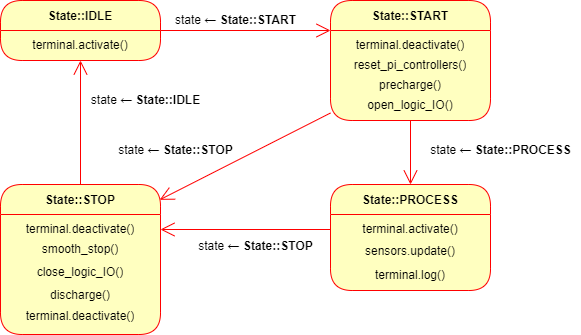
\includegraphics[width=10cm]
                { img/4_implementacio/state_machine.png }
            \caption{ Diagrama UML de la màquina d'estats finita.
             }
            \label{fms_uml}
        \end{figure}

        \paragraph{Main}
        {
            Representa el programa principal. En aquest mòdul s'hi defineix la
            funció principal del programa, en la que s'initzializen els
            registres AXI i es generen els \emph{threads} amb els
            \emph{handlers} de la màquina d'estats i la interfície de terminal,
            \lstinline{state\_loop()} i \lstinline{terminal\_loop()},
            respectivament.
        }
        
        \paragraph{State}
        { 
            En aquest mòdul s'han incorporat els mòduls relacionats amb la
            màquina d'estats. La instància de la classe \emph{State} representa
            un estat de la màquina d'estats. S'ha utilitzat una enumeració per
            descriure els estats. L'assignació de l'estat actual es realitza
            per mitjà de l'\lstinline{operator=()}. La seva implementació té en
            compte les possibles transicions i llança una excepció en el cas
            que es forci una transició que no és possible. El bucle que
            defineix la màquina d'estats s'ha implementat a la funció
            \lstinline{state_loop()}.

            \begin{figure}[!htb]
                \centering
                \captionsetup{justification=centering,margin=1.5cm}
                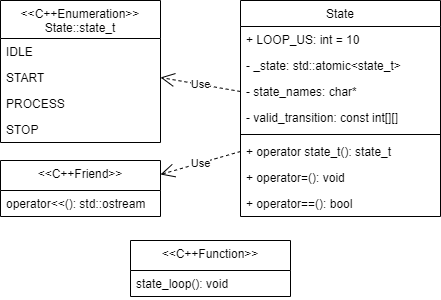
\includegraphics[width=7.5cm]
                    { img/4_implementacio/uml_state.png }
                \caption{ Diagrama UML del mòdul State.  }
            \end{figure}
        }

        \paragraph{Terminal} 
        { 
            En aquest mòdul s'hi defineix la interfície d'usuari amb el
            programa, en la qual l'usuari escriu les comandes per operar
            l'inversor. De manera paral·lela al mòdul State, s'ha creat una
            enumeració, en aquest cas amb les comandes possibles i una funció
            \lstinline{terminal_loop()}. 
            
            Així, les comandes \lstinline{Terminal::START} i
            \lstinline{Terminal::STOP} marquen el pas dels estats
            \lstinline{State::IDLE} a \lstinline{State::START} i de
            \lstinline{State::PROCESS} a \lstinline{State::STOP},
            respectivament. La comanda \lstinline{Terminal::EDIT} permet editar
            el valor dels registres AXI realitzant una cridada al programa de
            Linux $vi$. D'altra banda, les comandes \lstinline{Terminal::SPEED}
            i \lstinline{Terminal::TORQUE} permeten variar el valor de la
            velocitat i el parell durant l'estat \lstinline{State::PROCESS}.
            Finalment, \lstinline{Terminal::HELP} mostra un missatge d'ajuda i
            \lstinline{Terminal::UNKNOWN} és seleccionat en el cas que
            s'introdueixi una comanda no reconeguda.

            \begin{figure}[!htb]
                \centering
                \captionsetup{justification=centering,margin=1.5cm}
                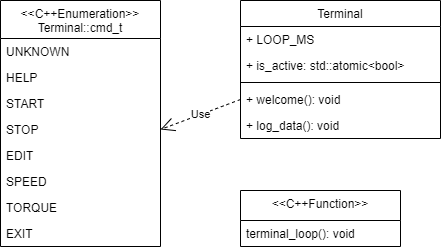
\includegraphics[width=7.5cm]
                    { img/4_implementacio/uml_terminal.png }
                \caption{ Diagrama UML del mòdul Terminal.  }
            \end{figure}
        }

        \paragraph{Register} 
        { 
            En aquest mòdul es defineixen, les classes Register i Sensor. La
            classe Register és una implementació a més alt nivell d'un registre
            del \ac{SoC}, en el que les lectures i les escriptures es
            converteixen de coma flotant a coma fixa i a l'inrevés, per a la
            seva interpretació per l'algorisme de control. La classe Sensor
            conté un Registre i en afegit incorpora la lògica per parar el
            funcionament de l'algorisme en cas que el sensor detecti que un
            registre sobrepassa un valor determinat, per exemple, de
            temperatura, voltatge o corrent.

            \begin{figure}[!htb]
                \centering
                \captionsetup{justification=centering,margin=1cm}
                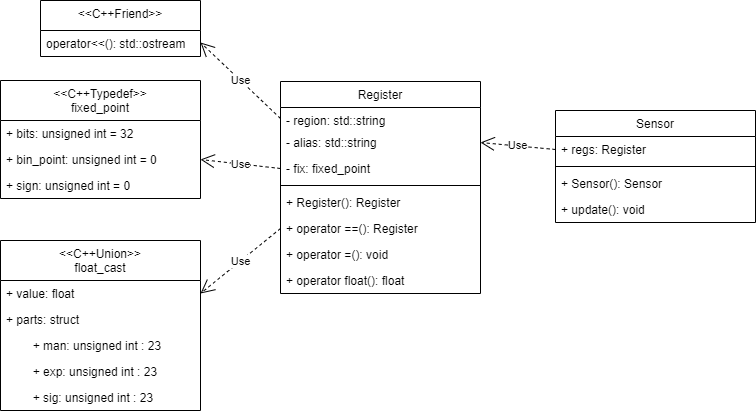
\includegraphics[width=11cm]
                    { img/4_implementacio/uml_register.png }
                \caption{ Diagrama UML de classes del mòdul Register.
                 }
            \end{figure}
        }

        \paragraph{Subroutines} 
        { 
            En aquest mòdul es defineixen les subrutines com funcions. Cada una
            d'elles realitza una sèrie de tasques, relacionades amb l'inversor.
            Aquestes subrutines no están implementades en el moment de
            l'escriptura de la memòria; sino que llençen una excepció
            notificant que no estan implementades. Les subrutines són les
            següents:

            \begin{itemize}

                \item \lstinline{void init_AXI_registers()}:
                    Initialitza els registres AXI de la lògica programable amb
                    els valors emmagatzemats a l'arxiu de paràmetres
                    \emph{param.txt}. Es crida quan s'inicia el programa i cada
                    cop que s'actualitza el contingut de \emph{param.txt}.

                \item \lstinline{void reset_pi_controllers()}:
                    Activa el senyal de reset dels blocs acumuladors dels
                    controladors PI. És una rutina bastant important que es
                    realitza.

                \item \lstinline{void precharge()}: 
                    Es comunica per bus CAN amb el microcontrolador de la placa
                    de precàrrega dels condensadors per notificar la intenció
                    d'iniciar el funcionament del motor i començar a
                    precarregar-los. Aquesta funció bloqueja la màquina
                    d'estats fins que acaba la precàrrega i rep el senyal
                    d'acabada.

                \item \lstinline{void discharge()}:
                    De manera semblant a la funció \lstinline{void precharge()}, estableix
                    comunicació amb el circuit de descàrrega, comença a
                    descarregar els condensadors i es bloqueja fins que acaba
                    la descàrrega, moment en el que rep el senyal d'acabada.

                \item \lstinline{void open_logic_IO()} i \lstinline{void close_logic_IO()}:
                    Aquestes funcions obren i tanquen els registres d'entrada i
                    de sortida de la lògica programable per iniciar el flux de
                    senyal a través de l'algorisme o per tancar-lo.
                    
                \item \lstinline{void change_speed(float speed)} i \lstinline{void change_torque(float torque)}:
                    Aquestes funcions canvien la consigna de velocitat i torque
                    de l'algorisme de control, respecivament, sempre que el
                    sistema es trobi en l'estat \lstinline{State::PROCESS}.

                \item \lstinline{void smooth_stop()}:
                    Realitza el protocol d'acabada suau per evitar que el
                    control finalitzi amb un esglaó.

            \end{itemize}
        } 

        \paragraph{Utils} 
        { 
            El mòdul Utils conté funcions i classes relacionades amb el flux del
            programa com són la classe Log i la funció exit program. En
            instanciar un objecte de la classe Log es mostra per pantalla
            informació, errors o advertències, i són habitualment llençades com
            com excepcions. En el mateix mòdul estàn definides les macros INFO,
            WARNING i ERROR per simplificar la seva implementació en el codi.
            D'altra banda, la funció \lstinline{exit_program()} comença a gestionar la
            sortida del programa en el cas que sigui possible. També és
            utilitzada per sobreescriure el \emph{handlers} dels senyals
            SIGNINT i SIGNTERM per evitar sortides del programa accidentals.
        
            \begin{figure}[!htb]
                \centering
                \captionsetup{justification=centering, margin=1.5cm}
                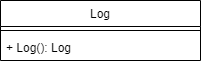
\includegraphics[width=3.8cm]
                    { img/4_implementacio/uml_log.png }
                \caption{ Diagrama UML de classes del mòdul Log. }
            \end{figure}
        } 
    }
}

\subsection{ Comunicació CAN }
{ 
    La comunicació pel bus CAN es realitza per mitjà del connector CAN de la
    placa Z-Turn. El packet SocketCAN del kernel de Linux proporciona els
    drivers necessaris per implementar diferents protocols de comunicació per
    CAN. La \ac{API} de SocketCAN per programar en C/C++, Linux-CAN, està basada en la Berkeley socket API, que
    té com avantatges ser independent del hardware i ser un estàndard prou
    utilitzat, amb la qual cosa es pot aprofitar l'extensa documentació al
    respecte per programar aplicacions com poden ser els populars servidors i
    clients TCP/IP \cite{can-utils} \cite{socketCAN}.

    S'ha dissenyat una prova per validar la implementació de CAN.
    Malauradament, el retràs en la comanda de la placa de la FPGA ha dificultat
    la validació de la comunicació per CAN, ja que la placa Cora Z-7 de la que
    es disposa no compta amb connector CAN i s'ha d'adaptar amb un hardware
    específic adicional (PmodCAN) que no està previst fer servir per la
    implementació de l'inversor.

    Per començar a desenvolupar amb la llibreria Linux-CAN, en un primer lloc,
    s'ha d'incloure la llibreria \lstinline{#include <linux/can.h>}. Un cop
    iniciat, s'ha de crear i configurar un descriptor de fitxer (\emph{file
    descriptor}) mitjançant la crida a la funció \lstinline{socket()},
    \lstinline{setsockopt()} i \lstinline{ioctl()}. Després de lligar el
    descriptor de fitxer a l'adreça del CAN amb \lstinline{bind()}, ja es pot
    començar a enviar dades amb les crides a \lstinline{write()} i
    \lstinline{read()}.
}